\section{Design of a Controller in State Space}\label{sec:SSController}
The aim of the controller is to maintain the system in equilibrium position, which means that the reference for each state is always zero. 

With this assumption a new state matrix can be created such that its poles are placed in the LHP and then the system becomes stable.This is done by adding a state feedback and a \si{3x1} gain matrix to the whole system, as seen in \figref{SSBlocksFeedback}.
%
\begin{figure}[H]
	\begin{tikzpicture}[ auto,
					thick,                         %<--setting line style
					node distance=1.5cm,             %<--setting default node distance
					scale=1,                     %<--|these two scale the whole thing
					every node/.style={scale=1}, %<  |(always change both)
					>=triangle 45 ]                %<--sets the arrowtype

	\draw%-----------------------------------------------------------------------------------------
	%Drawing Input/Output:
	node[shape=coordinate][](input1) at (0,0){}
	node[shape=coordinate][](output1) at (8,0){}
	%Drawing the Equation Blocks:   	
	node(A) at (4,-1.5) [block] {A} 
	node(B) at (1.5,0) [block] {B}
	node(C) at (6.5,0) [block] {C}
	node(int) at (4.5,0) [block] {\si{\int}} 
	node(K) at (3,-2.5) [block] {-K}	
	%Drawing the Sumation Blocks:	    	 	
	node(sum1) [sum, right of = B] {\si{\sum}}
	%Drawing the Feedback/Feedforward Nodes:    	
	node[shape=coordinate][](FeedbackNode) at (5.2,0){}  	
	node[shape=coordinate][](FeedbackNode2) at (5.6,0){} 
	
	;%---------------------------------------------------------------------------------------------

	%Joining the Blocks
	\draw[->](input1) -- node {u}(B);
	\draw[->](B) -- node {}(sum1);
	\draw[->](sum1) -- node {\si{\dot x}}(int);  	
	\draw[->](int) -- node {x}(C);
	\draw[-](C) -- node {y}(output1);

	\draw[->] (FeedbackNode) |- (A);
	\draw[->] (A)   -| (sum1);
	
	\draw[->] (FeedbackNode2) |- (K);
	\draw[-] (K)   -| (input1);

	%Drawing node(s) with \textbullet
	\draw%--------------------------------------------------------------
%	node at (input1)  [shift={(-0.08, -0.02 )}] {\large \textbullet}
	node at (output1) [shift={( 0.008, -0.04 )}] {\textbullet}
	;%------------------------------------------------------------------

\end{tikzpicture}
	\centering
	\caption{Block diagram with the state feedback}
\end{figure} \label{SSBlocksFeedback}
%
This new configuration gives a new equation for \si{\vec{\dot{x}}}:
%
\begin{flalign}
	\eq{\vec{\dot{x}}(\vec{t})}{(\vec{A}-\vec{B}\vec{K}) \cdot \vec{x}(\vec{t})}
	\label{xDotK} 
\end{flalign}
%
The objective is to find K such that the eigenvalues of \si{\vec{A}-\vec{B}\vec{K}} are placed at the LHP. This gain matrix can be found using the Matlab command K = place(A,B,P), where P is a vector containing the desired position of the new poles.

To choose the position of these poles two simulations are made for different values. In the first one the Cubli starts from equilibrium and a disturbance torque is applied while in the second one it starts from an initial angle different from \si{0\ rad} and with an initial acceleration.

\begin{minipage}{\linewidth}
	\begin{minipage}{0.45\linewidth}
		\begin{figure}[H]
			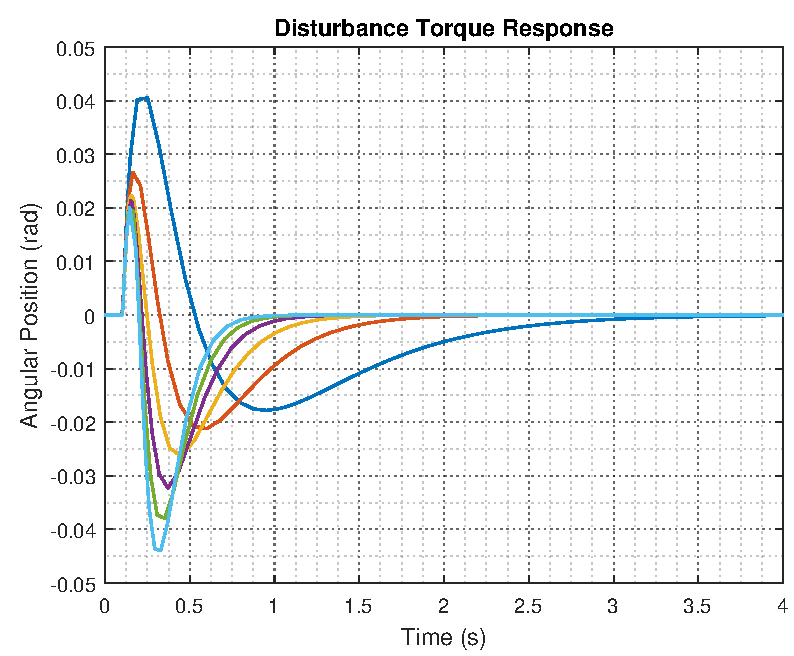
\includegraphics[scale=.5]{figures/disturbanceStateSpace}
			\centering
			\captionsetup{justification=centering}
			\captionof{figure}{Response of the system to a disturbance with different locations of poles}
			\label{disturbanceStateSpace}
		\end{figure}
	\end{minipage}
	\hspace{0.03\linewidth}
	\begin{minipage}{0.45\linewidth}
		\begin{figure}[H]\vspace{4mm}
			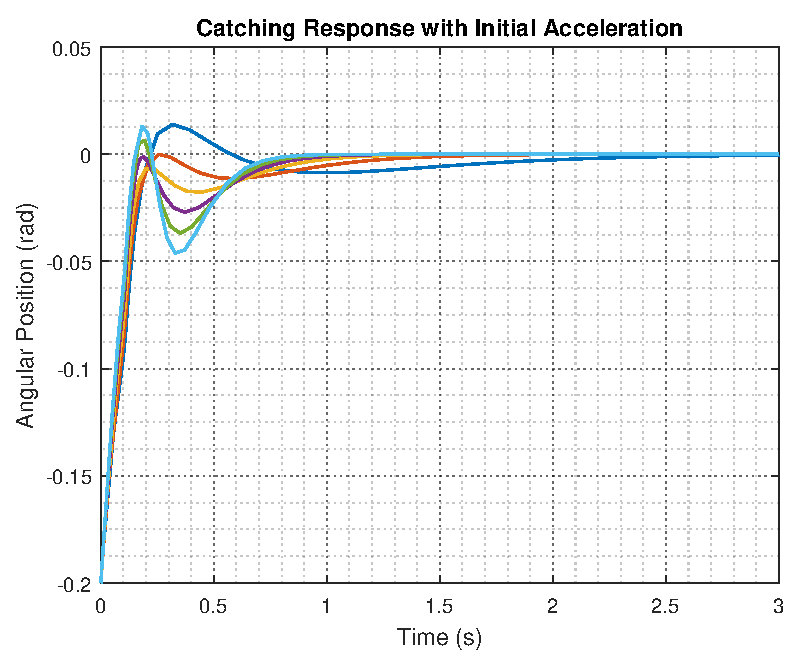
\includegraphics[scale=.5]{figures/catchingStateSpace}
			\centering
			\captionsetup{justification=centering}
			\captionof{figure}{Response starting from \si{0.2\ rad} and an initial velocity of the wheel with different locations of poles}
			\label{catchingStateSpace}
		\end{figure}
	\end{minipage}
\end{minipage}

The final combination of poles is \si{-6}, \si{-7} and \si{-10}, which gives the yellow responses in \figref{disturbanceStateSpace} and \figref{catchingStateSpace}. This seems a good option since its response is quite fast but not with too much overshoot. The gain matrix for this combination results in the following:
%
\begin{equation}  \label{controllerSS}
	\vec{K} = 
	\begin{bmatrix}
		-2,3021 & -0,227 & -0,0039 \\
	\end{bmatrix}
\end{equation}
%